\chapter{Исследовательский раздел}

\section{Сравнение результатов, полученных методом, с результатами других методов}

Для достижения данной цели были использованы обученные веса для сети, которые были получены в аналитическом разделе. Затем было проведено устранение размытия. Далее было вычислено значение метрики \textit{PSNR} для оценки эффективности разработанного метода.

На рисунке \ref{fig:comparation} представлено изображение, которое было использовано для проведения оценки эффективности метода.
\begin{figure}[H]
    \centering
    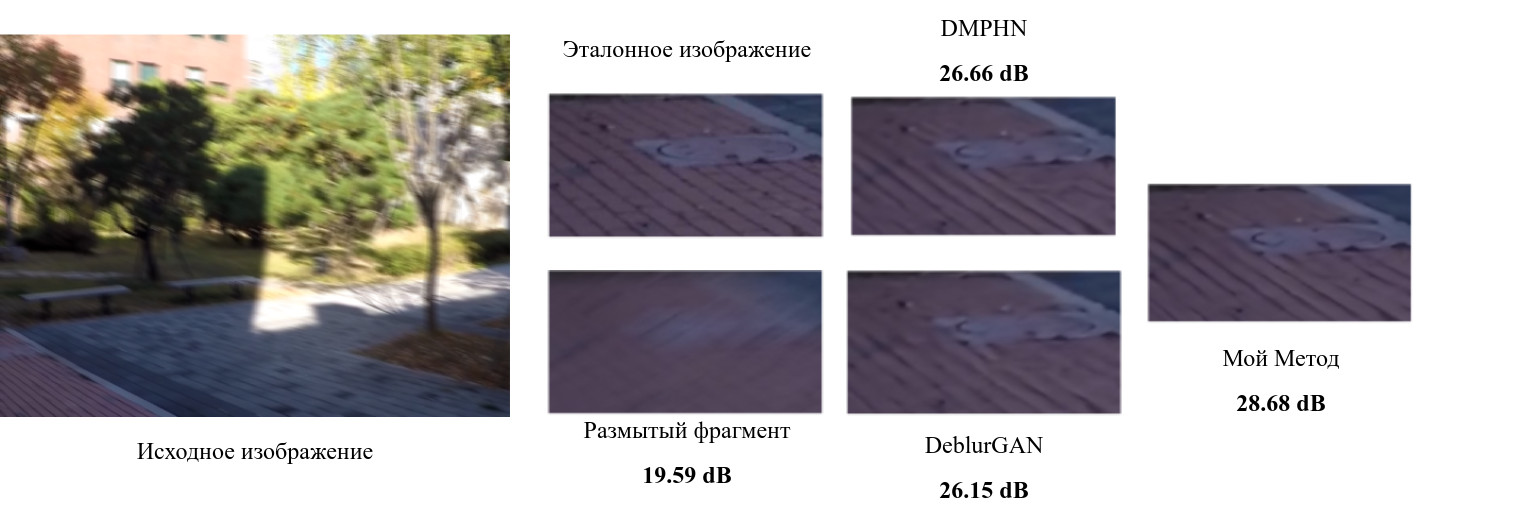
\includegraphics[width=1.0\textwidth]{assets/comparation.png}
    \caption{Изображение для оценки эффективности разработанного метода}
    \label{fig:comparation}
\end{figure}

В итоге полученное значение \textit{PSNR} составило 28.68 децибела, что показывает значительное улучшение работы разработанного метода, в то время как для выбранное изображение \textit{DMPHN} дает 26.66, а \textit{DeblurGAN} - 26.15.

\section{Проведение тестирования метода на корпусе данных}

Для достижения данной цели был выбран еще один корпус данных \textit{HIDE}, изображения которого не присутствовали в обучающем наборе данных, а также 1/3 часть изображений из корпуса данных \textit{GoPro}, которые также не использовались при обучении сети. Для сравнения эффективности метода, аналогично предыдущему подразделу, было проведено устранение размытия с использованием обученных весов сети, после чего было выполнено сравнение метрик \textit{PSNR} и \textit{SSIM} относительно эталонного изображения и изображения, полученного из сети. Затем было рассмотрено среднее значение метрик \textit{PSNR} и \textit{SSIM}. В данном исследовании был проведен сравнительный анализ средних значений метрик \textit{PSNR} и \textit{SSIM} относительно изображений, использованных для тестирования сети.

В таблице (\ref{tab:metric-comparation}) представлен средние значения объективных метрик \textit{PSNR} и \textit{SSIM} относительно корпусов данных \textit{GoPro} и \textit{HIDE}.

\begin{table}[H]
    \centering
    \caption{Средние значения объективных метрик, полученные с использованием обученных весов сети, относительно корпусы данных \textit{GoPro} и \textit{HIDE}}
    \label{tab:metric-comparation}
    \begin{tabular}{|p{4cm}|p{2cm}|p{2cm}|p{2cm}|p{2cm}|}
        \cline{2-5}
        \multicolumn{1}{c|}{\myrule}                  & \multicolumn{2}{|c|}{GoPro} & \multicolumn{2}{|c|}{HIDE} \\ \hline
        \myrule \backslashbox[4.4cm]{Метод}{Метрика}   & PSNR  & SSIM   & PSNR  & SSIM \\ \hline
        \myrule \textbf{DeblurGAN}                     & 31.10 & 0.942  & 28.94 & 0.915 \\ \hline
        \myrule \textbf{DMPHN}                         & 31.20 & 0.940  & 29.09 & 0.924 \\ \hline
        \myrule \textbf{MPRNet}                     & 32.66 & 0.959  & 30.96 & 0.939 \\ \hline
    \end{tabular}
\end{table}

Как видно из полученных результатов метрик \textit{PSNR} и \textit{SSIM}, разработанный метод не только в деталях демонстрирует хорошие результаты, но также по значению объективных метрик превосходит другие методы и показывает наилучшие результаты.

\section{Эффективность метода размытия на реальных изображениях}

Для достижения этой цели было выбрано изображение из корпуса данных \textit{RealBlur} \cite{rim2020real}. Все изображения в этом корпусе сняты с помощью мобильных камер или фотоаппаратов. Разрешение этих изображений различно, и изображение делится на две категории: 

\begin{enumerate}
    \item \textit{RealBlur-R};
    \item \textit{RealBlur-J}. 
\end{enumerate}
    
Изображения в категории \textit{RealBlur-R} создавались в автономном режиме путем применения к необработанным изображениям операций по балансу белого, демозакладке и уменьшению шума, а изображения в категории \textit{RealBlur-J} формировались с помощью снятых изображений камеры в формате \texit{JPEG}.

Было проведено тестирование на обеих этих категории, результат средние значение объективных метриков, полученного с помощью обучениеми весами сети на данные из корпуса данных \textit{GoPro}, представлен на таблице \ref{tab:metric-comparationrealblur}.

\begin{table}[H]
    \centering
    \caption{Средние значения объективных метрик, полученные с использованием обученных весов сети, относительно корпуса данных \textit{RealBlur}}
    \label{tab:metric-comparationrealblur}
    \begin{tabular}{|p{4cm}|p{2cm}|p{2cm}|p{2cm}|p{2cm}|}
        \cline{2-5}
        \multicolumn{1}{c|}{}                  & \multicolumn{2}{|c|}{RealBlur-R} & \multicolumn{2}{|c|}{RealBlur-J} \\ \hline
        \backslashbox[4.4cm]{Метод}{Метрика}   & PSNR  & SSIM   & PSNR  & SSIM \\ \hline
        \textbf{DeblurGAN}                     & 33.79 & 0.903  & 33.79 & 0.903 \\ \hline
        \textbf{DMPHN}                         & 35.70 & 0.948  & 35.70 & 0.948 \\ \hline
        \textbf{MPRNet}                     & 35.99 & 0.952  & 35.99 & 0.952 \\ \hline
    \end{tabular}
\end{table}

Исходя из полученных значений, можно сделать вывод, что метод хорошо справляется с изображениями из реального мира, поскольку корпус данных \textit{RealBlur} содержит изображения, снятые с разных видов фотоаппаратов и разных разрешений. Однако, если обучить сеть на этих данных, то можно получить лучшие результаты.

\section*{Вывод}

В данном разделе был проведен сравнительный анализ разработанного метода относительно других методов. Было проведено тестирование сети на реальных изображениях и сгенерированных размытых изображениях. В итоге были составлены таблицы с полученными результатами. По полученным данным можно сделать вывод, что метод хорошо справляется с изображениями, снятыми с разных видов фотоаппаратов и различных разрешений. Однако, чтобы гарантировать работу метода на различных видах изображений, лучшим способом является обучение сети на этих изображениях.